\documentclass[english,14pt]{beamer}
\usetheme{EastLansing}
\usecolortheme{spruce}

\usepackage{xcolor}
\usepackage{listings}
\usepackage{courier}
\usepackage{graphicx}
\usepackage{amsmath}
\usepackage{algorithm2e}
\usepackage{multicol}
\usepackage{hyperref}
\usepackage{textcomp}

% http://mirrors.ibiblio.org/CTAN/macros/latex/contrib/datetime2/datetime2.pdf
\usepackage{babel}
\usepackage[useregional]{datetime2}

% https://tex.stackexchange.com/questions/42619/x-mark-to-match-checkmark
\usepackage{pifont}% http://ctan.org/pkg/pifont

%% https://stackoverflow.com/questions/1435837/how-to-remove-footers-of-latex-beamer-templates
%%gets rid of bottom navigation bars
%\setbeamertemplate{footline}[page number]
%
%gets rid of navigation symbols
\setbeamertemplate{navigation symbols}{}


\usefonttheme[onlymath]{serif}

\definecolor{mGreen}{rgb}{0,0.6,0}
\definecolor{mGray}{rgb}{0.5,0.5,0.5}
\definecolor{mPurple}{rgb}{0.8,0,0.82}
\definecolor{backgroundColour}{rgb}{0.95,0.95,0.92}
\definecolor{lightBlue}{rgb}{0.1, 0.1, 0.8}
\definecolor{darkGreen}{rgb}{0, 0.39, 0}

\newcommand\red[1]{{\color{red} #1}}
\newcommand\green[1]{{\color{green} #1}}
\newcommand\blue[1]{{\color{blue} #1}}
\newcommand\darkGreen[1]{{\color{darkGreen} #1}}

\newcommand{\cmark}{\ding{51}}%
\newcommand{\xmark}{\ding{55}}%

\lstdefinestyle{CStyle}{
    backgroundcolor=\color{backgroundColour},   
    commentstyle=\color{mGreen},
    keywordstyle=\color{magenta},
    numberstyle=\tiny\color{mGray},
    stringstyle=\color{mPurple},
    basicstyle=\footnotesize,
    breakatwhitespace=false,         
    breaklines=true,                 
    captionpos=b,                    
    keepspaces=true,                 
    numbers=left,                    
    numbersep=5pt,                  
    showspaces=false,                
    showstringspaces=false,
    showtabs=false,                  
    tabsize=2,
    language=Python
}

\lstdefinestyle{pseudo}{
        basicstyle=\ttfamily\footnotesize,
        keywordstyle=\color{lightBlue},
        morekeywords={BEGIN,END,IF,ELSE,ENDIF,ELSEIF,PRINT,WHILE,RETURN,ENDWHILE,DO,FOR,TO,IN,ENDFOR,BREAK,INPUT,CONDITIONS},
        morecomment=[l]{//},
        commentstyle=\color{mGreen}
}

\lstset{basicstyle=\footnotesize\ttfamily,breaklines=true}
\lstset{framextopmargin=50pt,tabsize=2}

\title{ENGG1003 - Monday Week 12}
\subtitle{The C programming language \& \\ version control with Git}
\author{Brenton Schulz and Steve Weller}
\institute{University of Newcastle}
%\date{\today}
\date{24 May 2021}

% following is a bit of a hack, but forces page numbers (technically: frame numbers) to run 1,2,3,... 
% with titlepage counting as frame 1

\addtocounter{framenumber}{1}
\titlepage

\begin{document}

\begin{flushleft}
{\scriptsize Last compiled:~\DTMnow}
\vspace*{-5mm}
\end{flushleft}
\framebreak

%==============================================================

\begin{frame}[fragile]

\frametitle{Lecture overview}
\begin{enumerate}
	\item Context
	\begin{itemize}
		\item ENGG1003
		\item what is C?
		\item do we even need C?
	\end{itemize}
	\item[]
		\item C programming language
	\begin{itemize}
		\item features and philosophy
		\item key language details of C
	\end{itemize}
	\item[]
	\item Version control with Git
		\begin{itemize}
			\item principles
			\item practical demonstration (live demo by Brenton)
		\end{itemize}		
\end{enumerate}

\end{frame}

%==============================================================

\begin{frame}[fragile]

\frametitle{$1)$ Context}

\begin{itemize}
	\item Recall from last week\ldots
	\item[]
	\item $\leq$ 2020, ENGG1003 used \red{\emph{MATLAB}} and \red{\emph{C}}
	\begin{itemize}
		\item \textbf{from 2021, ENGG1003 uses Python only}
		\item \ldots yet some students will use MATLAB \&/or C in later courses
	\end{itemize}
	\item[]
	\item Thursday week 11: overview of MATLAB
	\item[]
	\item today's lecture: overview of C
\end{itemize}

\end{frame}

%==============================================================

\begin{frame}[fragile]

\frametitle{What is C?}

\begin{itemize}
	\item C is a general-purpose, high-level programming language
	\begin{itemize}
		\item other high-level languages: Python, MATLAB, Java, C++, FORTRAN, \ldots
	\end{itemize}
	\item C has been around since early-1970s and still \emph{very} popular
	\begin{itemize}
		\item IEEE language ranking 2020: \#1:~Python \textbf{\#3:~C} \\ \#10:~MATLAB
%		\item[] \href{https://spectrum.ieee.org/static/interactive-the-top-programming-languages-2020}{https://spectrum.ieee.org/static/interactive-the-top-programming-languages-2020}
	\end{itemize}
	\item C is native language of Linux, Microsoft Windows, OS X, iOS, \& Android kernels
	\item even Python language is written in C
	\item \textbf{C language constructs map efficiently to computer hardware (machine instructions)}
\end{itemize}

\end{frame}

%==============================================================

\begin{frame}[fragile]

\frametitle{Do we even need C?}

\begin{itemize}
	\item \textbf{C is \emph{not} assessable in ENGG1003}
	
	\item[]
	
	\item BUT\ldots C is currently used in some courses in some Engineering programs:
	\begin{itemize}
		\item Aerospace Systems, Computer Systems, Electrical, Mechatronics and Medical Engineering
	\end{itemize}
	
	\item[]
	\item key courses which use C language:
	\begin{itemize}
		\item ELEC2720, ELEC3730, AERO3600, MCHA3400, MCHA3500
		\item common theme of all these courses is \red{\emph{embedded systems}}
	\end{itemize}

\end{itemize}
\end{frame}

%==============================================================

\begin{frame}[fragile]

\frametitle{Embedded systems}

\begin{itemize}
	\item embedded system: coupled hardware and software designed for a \emph{specific task}
	\item[]
	\item eg: washing machine
	\begin{itemize}
		\item inputs: buttons, water-level, water temperature
		\item output: LED display, motor control
		\item control unit: microprocessor \& memory		
	\end{itemize}
	\item[]
	\item \emph{many} other examples: smart TVs, gaming consoles, medical devices, WiFi routers,  automotive \ldots
	\item[]
	\item \textbf{C language is well-suited to tight coupling of hardware and software in embedded systems}
\end{itemize}

\end{frame}

%==============================================================

\begin{frame}[fragile]

\frametitle{$2)$ C programming language}

Quick recap of \red{\emph{computer language hierarchy}}, week~1:

\begin{itemize}
	\item \textbf{machine code}
	\begin{itemize}
		\item a microprocessor can only understand machine code
		\item eg: one instruction for an x86-based processor:
		\item[] 0110 0110 1000 0011 1100 0000 0000 1010
		\item very processor-specific!
	\end{itemize}
	
	\item \textbf{assembly language}

	\begin{itemize}
		\item human-readable abbreviations (``mnemonics'')
		\item eg: machine code
		\item[] 0110 0110 1000 0011 1100 0000 0000 1010
		\item same instruction in assembly language
		\item[] \texttt{ADD AX, 10}
		\item very processor-specific
	\end{itemize}
	
\end{itemize}

\end{frame}

%==============================================================

\begin{frame}[fragile]

\frametitle{}

\begin{itemize}
	\item \textbf{high-level languages} eg: C, Python, MATLAB \ldots

	\begin{itemize}
		\item human-readable text-based code
		\item increased complexity of each high-level instruction
		\item eg: machine code
		\item[] 0110 0110 1000 0011 1100 0000 0000 1010
		\item same instruction in assembly language
		\item[] \texttt{ADD AX, 10}
		\item same instruction in C
		\item[] \texttt{x = x + 10;}
		\item \emph{not} processor-specific (that's a good thing)
	\end{itemize}
	
	% https://medium.com/@vietkieutie/what-happens-when-you-type-gcc-main-c-2a136896ade3
	
	\item \red{\emph{compilation process}} converts source code (eg: C) to machine code
	\begin{itemize}
		\item source code $\rightarrow$ pre-processor $\rightarrow$ compiler $\rightarrow$ assembler $\rightarrow$  linker $\rightarrow$  machine code (``executable'')
	\end{itemize}
	
\end{itemize}

\end{frame}

%==============================================================

\begin{frame}[fragile]

\frametitle{Hello, World!  \ldots in the C language}

\begin{lstlisting}[style=CStyle,basicstyle=\small]
#include <stdio.h>

int main()
{
    printf("Hello, World!\n");
    return 0;
}
\end{lstlisting}

\begin{itemize}
	\item line 1: header file \texttt{stdio.h}, like Python \texttt{import}
	\item line 3: function definition for \texttt{main()}, returns \texttt{int}
	\item line 5: formatted print, \verb+\n+ means ``newline''
	\item line 6: returns ``all good'' (error-free) message
	\item lines 4 \& 7: \{$\cdot$\} begin/end of function \texttt{main()}
\end{itemize}

\end{frame}

%==============================================================

\begin{frame}[fragile]

\frametitle{Hello, World! program in C and assembly}

\begin{figure}[ht]
	\centering
	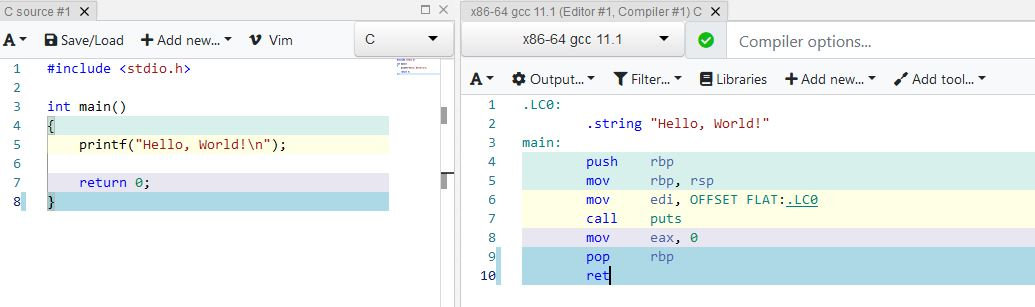
\includegraphics[width=\textwidth]{figures/Cvsx86assembly}
\end{figure}

\begin{itemize}
	\item left panel: C program
	\item right panel: corresponding assembly language code for 64-bit Intel x86
	\begin{itemize}
		\item x86 instructions:~\texttt{push, mov, call, pop, ret}
	\end{itemize}
	\item try it yourself at: \href{https://godbolt.org/}{https://godbolt.org/}
\end{itemize}

\end{frame}

%==============================================================

\begin{frame}[fragile]

\frametitle{}

\begin{figure}[ht]
	\centering
	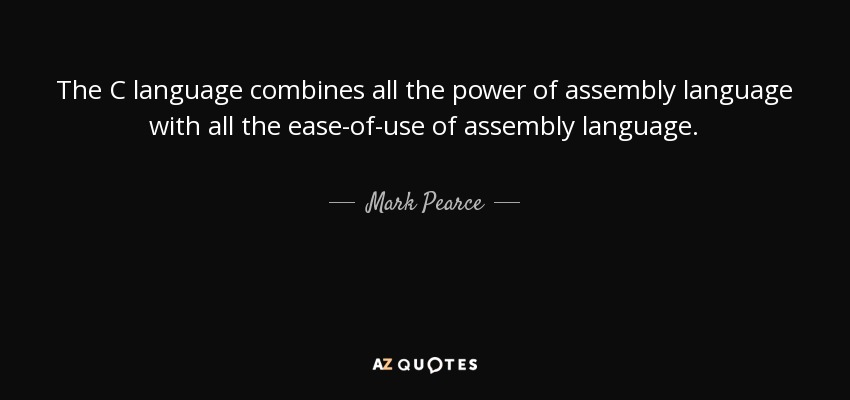
\includegraphics[width=\textwidth]{figures/Cquote}
\end{figure}

\end{frame}

%==============================================================

\begin{frame}[fragile]

\frametitle{}

\begin{figure}[ht]
	\centering
	
\includegraphics[width=\textwidth]{figures/LCTHW}
\end{figure}

\href{https://learncodethehardway.org/c/}{https://learncodethehardway.org/c/}	

\end{frame}

%==============================================================

\begin{frame}[fragile]

\frametitle{OnlineGDB: browser-based C development}

\begin{figure}[ht]
	\centering
	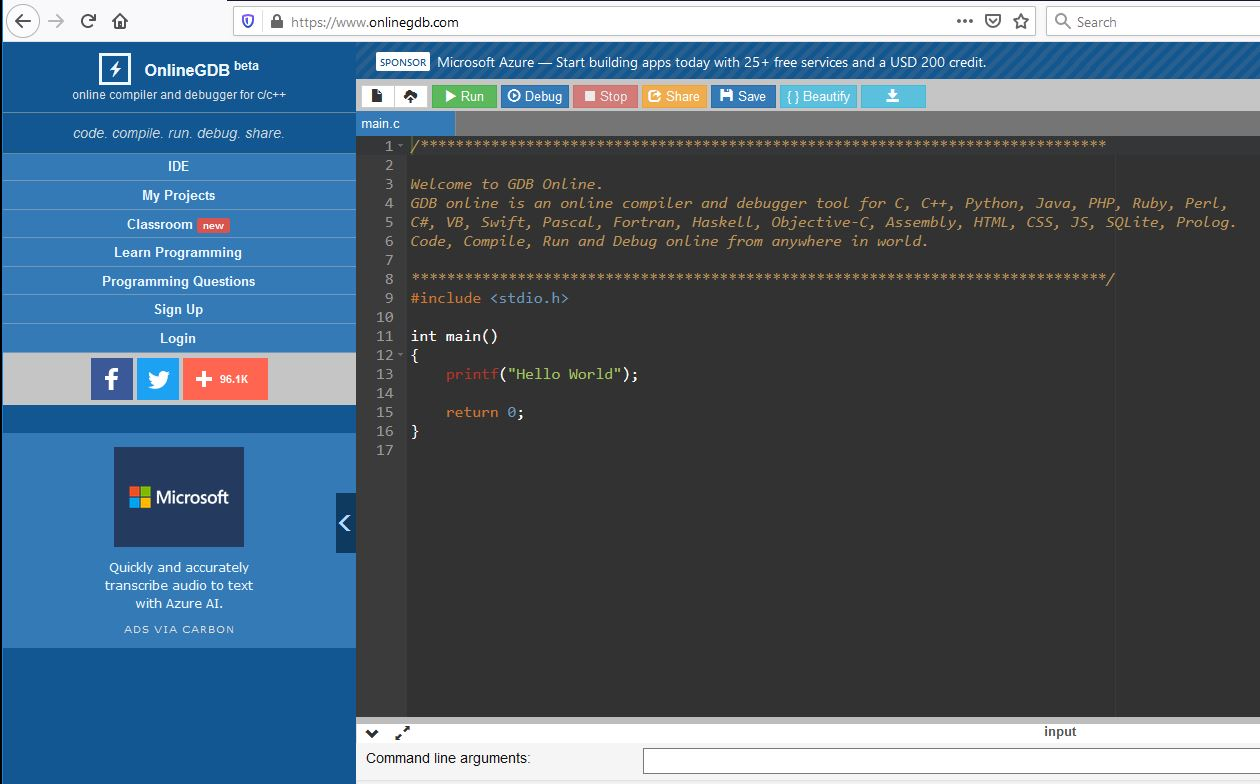
\includegraphics[width=.7\textwidth]{figures/OnlineGDB}
\end{figure}

edit, compile and run simple C programs with no setup! \\
\href{https://www.onlinegdb.com/}{https://www.onlinegdb.com/}

\end{frame}


%==============================================================

\begin{frame}[fragile]

% https://www.programiz.com/c-programming/examples/print-integer

\frametitle{C program: read and print an integer}
\vspace*{-3mm}
\begin{lstlisting}[style=CStyle,basicstyle=\footnotesize]
#include <stdio.h>
int main() {   
    int number;
   
    printf("Enter an integer: ");  
    
    // reads and stores input
    scanf("%d", &number);

    // displays output
    printf("You entered: %d", number);
    
    return 0;
}
\end{lstlisting}
\vspace*{-3mm}
\begin{itemize}
	\item line 3: need to ``declare'' variables before use
	\item line 8: \texttt{scanf()} reads from keyboard, \texttt{\&number} means ``address of variable \texttt{number} in memory''
\end{itemize}

\end{frame}

%==============================================================

\begin{frame}[fragile]

% https://www.programiz.com/c-programming/examples/sum-natural-numbers

\frametitle{C program: sum of integers using a loop}
\vspace*{-3mm}
\begin{lstlisting}[style=CStyle,basicstyle=\footnotesize]
#include <stdio.h>
int main() {
    int n, i, sum = 0;

    printf("Enter a positive integer: ");
    scanf("%d", &n);

    for (i = 1; i <= n; ++i) {
        sum += i;
    }

    printf("Sum = %d", sum);
    return 0;
}
\end{lstlisting}
\vspace*{-3mm}
\begin{itemize}
	\item lines 8--10: iterate with \texttt{for} loop
	\item[] initialise \texttt{i} at 1; continue looping if \texttt{i} $\leq$ \texttt{n} is true; update \texttt{i} $=$ \texttt{i} $ + 1$ after each iteration of loop body
\end{itemize}

\end{frame}

%==============================================================

\begin{frame}[fragile]

% https://www.programiz.com/c-programming/examples/power-number

\frametitle{C program: power of a number $\mathrm{base}^\mathrm{exp}$}
\vspace*{-3mm}
\begin{lstlisting}[style=CStyle,basicstyle=\scriptsize]
#include <stdio.h>
int main() {
    int base, exp;
    long result = 1;
    printf("Enter a base number: ");
    scanf("%d", &base);
    printf("Enter an exponent: ");
    scanf("%d", &exp);

    while (exp != 0) {
        result *= base;
        --exp;
    }
    printf("Answer = %ld", result);
    return 0;
}
\end{lstlisting}
\vspace*{-3mm}
\begin{itemize}
	\item lines 10--13: \texttt{while} loop, continues while \texttt{exp} $\neq 0$
	\item line 11: \texttt{result = result * base}
	\item line 12: decrement \texttt{exp}, ie: \texttt{exp = exp - 1}
\end{itemize}

\end{frame}

%==============================================================

\begin{frame}[fragile]

\frametitle{$3)$ Version control with Git}

Programming projects often give rise to two problems:
\begin{enumerate}
	\item programmers want to ``roll back'' to earlier code
	\begin{itemize}
		\item after trying an unsuccessful idea, sometimes faster to load up working code from the past and go 	from there
	\end{itemize}
	\item multiple people contribute to the same project. How should their changes be ``merged'' into some
kind of ``master'' code listing?
\end{enumerate}

%\vspace*{5mm}

\begin{itemize}
	\item \red{\emph{version control systems}} solve both problems
	\item most widely used version control system is \red{\emph{Git}}
\end{itemize}

\end{frame}

%==============================================================

\begin{frame}[fragile]

\frametitle{}

\vspace*{-5mm}

\begin{figure}[ht]
	\centering
	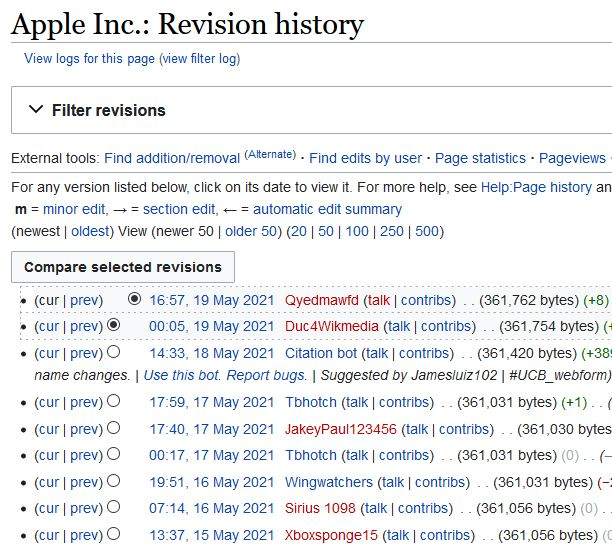
\includegraphics[width=.45\textwidth]{figures/AppleWiki}
\end{figure}

\vspace*{-5mm}

\begin{itemize}
	\item Wikipedia records history of changes
	\item every time an edit is made, it's recorded in history, even if that change is later reverted
	\item possible to go back in time to look at that page, at any point in its history
\end{itemize}

\end{frame}

%==============================================================

\begin{frame}[fragile]

\frametitle{Common Git terms}

\begin{itemize}
	\item \textbf{Repository (repo)}
	\begin{itemize}
		\item store of all the different pieces of the project
		\item collection of files $+$ history of changes made to those files
	\end{itemize}
	\item[]
	\item \textbf{Commit}
	\begin{itemize}
		\item captures a snapshot of the project
	\end{itemize}
	\item[]
	\item \textbf{Push}
	\begin{itemize}
		\item upload local repository content to a remote repository
	\end{itemize}
	\item[]
	\item \textbf{Pull}
	\begin{itemize}
		\item  update the local version of a repository from a remote
	\end{itemize}
\end{itemize}

\end{frame}

%==============================================================

\begin{frame}[fragile]

\frametitle{Practical demonstration of Git}

\begin{itemize}
	\item over to you, Brenton \ldots
\end{itemize}

% https://chris.beams.io/posts/git-commit/
\begin{figure}[ht]
	\centering
	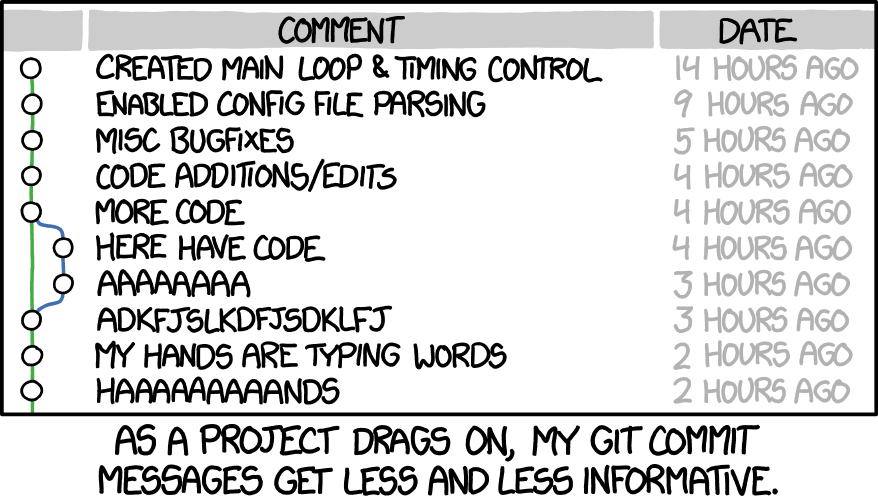
\includegraphics[width=.8\textwidth]{figures/git_commit_2x}
\end{figure}

\end{frame}

%==============================================================

\begin{frame}[fragile]

\frametitle{Next steps}
\begin{itemize}
	\item[]\textbf{C is \emph{not} assessable in ENGG1003}
	\item[]
	\item getting started with C, if you need it \emph{for later courses}		
	\item[]
	\item Code::Blocks integrated development environment
	\begin{itemize}
		\item \href{https://www.codeblocks.org/downloads/binaries/}{https://www.codeblocks.org/downloads/binaries/}
		\item runs on various platforms:
		\begin{itemize}
			\item Windows XP / Vista / 7 / 8.x / 10
			\item Linux 32- and 64-bit
			\item Mac OS X
		\end{itemize}
	\end{itemize}
	\item[] {\tiny C code examples Copyright \copyright 2020 Parewa Labs Pvt. Ltd.}
\end{itemize}
	
\end{frame}

\end{document}